\section{INTRODUÇÃO}

As atividades agropecuárias têm grande relevância na economia brasileira. Segundo um estudo realizado pelo Centro de Estudos Avançados em Economia Aplicada (CEPEA), da Esalq/USP, a parcela da participação do agronegócio no PIB brasileiro foi de $20,5\%$ em $2019$ e, em $2020$, este percentual chegou a $26,6\%$ \cite{cepea21_2}. De acordo com o último Censo Agropecuário, entre $2006$ e $2017$, houve um acréscimo de cerca de $5,8\%$ na área total dos estabelecimentos agropecuários e, tanto a área total quanto a produção agrícola e pecuária apresentaram um considerável crescimento \cite{ibge19_2}.

No entanto, o ambiente no qual se desenvolvem as atividades agropecuárias apresenta elevado risco e significativa incerteza. Essa insegurança se deve, principalmente, às instabilidades climáticas e ameaças sanitárias, que podem afetar a produção, ou à razões de mercado, como variações das taxas de câmbio e juros, ou a condições ligadas ao ambiente de negócios, tais como alterações em marcos regulatórios e em políticas públicas. Todas essas variáveis, relacionadas aos mercados agropecuários, geram variações na renda do setor, que são comumente enfrentadas por meio de políticas de apoio à gestão de riscos \cite{brasil18_2}.

O gerenciamento de riscos agropecuários pode ocorrer de diversas maneiras. No entanto, a contratação de seguro rural é uma das formas mais usuais. Essa modalidade de seguro atua no sentido de amenizar as perdas e possibilitar a recuperação da capacidade financeira do produtor na ocorrência de sinistros. O seguro rural propicia um ambiente mais favorável ao desenvolvimento das atividades agropecuárias, pois proporciona a garantia do fluxo de renda, favorece um aumento da área plantada e facilita a obtenção de financiamento. Além disso, se mostra um instrumento que possibilita o compartilhamento do risco da agropecuária com outros agentes e setores econômicos \cite{brasil19_2}.

É importante destacar que o mercado de seguro rural não se consolida sem a participação do Estado. Destacam-se problemas, como os elevados investimentos e custos administrativos, a possibilidade de riscos catastróficos, a forte influência do risco moral e da seleção adversa na formação das carteiras, como fatores que limitam a eficiência da iniciativa privada na oferta de produtos. Nesse sentido, o poder público é demandado a interferir no mercado, seja atuando diretamente como seguradora, seja criando programas que estimulem a oferta e a demanda por produtos de seguro (BRASIL, 2019a). 

% Esses dois estão ok...

Considerando a relevância do seguro rural no setor agropecuário, este estudo tem como objetivo analisar a distribuição espacial de dados multivariados do seguro rural nos municípios brasileiros entre os anos de $2006$ e $2019$. Além disso, busca-se investigar a presença de padrões de distribuição espacial nos dados, mais especificamente, se há presença de dependência ou heterogeneidade espacial. Por fim, este trabalho pretende fornecer informações que possam contribuir para o debate em torno do aperfeiçoamento do sistema de seguro rural no Brasil. Para alcançar tais objetivos, o trabalho faz uso da Análise de Componentes Principais (ACP) para reduzir a dimensionalidade dos dados e da Análise Exploratória de Dados Espaciais (AEDE) para investigar a presença de padrões de distribuição espacial. São utilizados dados oriundos dos Censos do Seguro Rural, compilados pelo Ministério da Agricultura, Pecuária e Abastecimento \cite{brasil21_2}.

O trabalho estrutura-se da seguinte forma: na seção $2$ descreve a metodologia utilizada neste estudo, a fonte dos dados e os recursos computacionais. A seção $3$ discute os resultados obtidos. Por fim, a seção $4$ traz as considerações finais. 
%na seção $2$ é apresentado uma revisão de literatura a respeito do seguro rural no Brasil, assim como a Análise de Componentes Principais e a Análise Exploratória de Dados Espaciais. A 

\section{MATERIAL E MÉTODOS}\label{methods}

\subsection{Fonte dos dados e recursos computacionais utilizados}

% Dados
Foram utilizados dados anuais referentes a apólices de seguro rural dos municípios brasileiros a partir do ano de $2006$ até o ano de $2019$. As variáveis utilizadas na análise são apresentadas na Tabela \ref{tab_variaveis}. Para todas as variáveis, foi utilizado o nível de agregação municipal. Nos casos em que as informações disponíveis eram referentes a outras localidades, como distritos, fazendas e vilarejos, tais informações foram atribuídas aos municípios correspondentes. 

\begin{small}
\begin{table}[H]
\caption{Descrição das variáveis utilizadas.}\label{tab_variaveis}
 \begin{center}
\begin{tabular}{ll}
\hline 
Sigla & Variável  \tabularnewline
\hline 
ap\_contrat    & Total de apólices contratadas                         \\
t\_segurado    & Soma da importância segurada (R\$ milhão)             \\
soma\_premio   & Soma dos prêmios (R\$ milhão)                         \\
t\_subvencao   & Total de subvenção (R\$ milhão)                       \\
inde\_pagas    & Soma das indenizações pagas (R\$ milhão)              \\
tx\_media      & Taxa média aplicada às apólices                       \\
ap\_indeniz    & Número de apólices indenizadas                        \\ 
%\tabularnewline
\hline 
\vspace{0.1cm}
\footnotesize{Fonte: Elaboração própria}
%\end{tabular}
\end{tabular}
\end{center}
\end{table}
\end{small}
	
% Fonte dos Dados 
Os dados sobre seguro rural são provenientes do endereço eletrônico do Ministério da Agricultura, Pecuária e Abastecimento (MAPA). Os dados que contêm atributos geográficos, como a posição e o formato do território brasileiro, foram obtidos no endereço eletrônico do Instituto Brasileiro de Geografia e Estatística (IBGE, 2020).
	
%Padronização
Como as variáveis estão em diferentes escalas e, com isto, possuem diferentes variâncias, foi realizada a padronização das variáveis para que tais fatores não interferissem na análise. Tal padronização foi efetuada subtraindo-se de cada observação a média de sua respectiva variável e dividindo-se, posteriormente, pelo desvio padrão da variável.

% Linguagem de programação 
Esse estudo foi realizado com a linguagem de programação \textit{Python} \cite{python17_2}, utilizando-se a interface \textit{Jupyter} \cite{jupyter17_2}, \cite{perez07_2} \cite{kluyver19_2}.
Além disso, as seguintes bibliotecas foram utilizadas: 
\textit{Pandas} \cite{mckinney10_2}, para a manipulação de dados,
\textit{NumPy} \cite{walt11_2}, que possibilita computação numérica com \textit{Python},
\textit{Matplotlib} \cite{hunter07_2} e \textit{Seaborn} \cite{waskom14_2}, que são bibliotecas para a criação de gráficos e 
\textit{jenkspy} para a utilização do algoritmo Fisher Jenks \cite{jenks77_2}. 
A análise de componentes principais foi realizada através da biblioteca \textit{sklearn} e as bibliotecas \textit{Geopandas} \cite{jordahl14_2} e \textit{PySAL} \cite{rey07_2} possibilitaram a análise espacial \footnote{Os códigos utilizados na análise estão disponíveis no \textit{GitHub} e os link estão no Apêndice B.}.

%Nesse trabalho, foi utilizada a análise exploratória de dados espaciais com o objetivo de avaliar a distribuição espacial do seguro rural nos municípios brasileiros no período de $2006$ a $2019$. Inicialmente, foi realizada uma análise exploratória dos dados de forma a auxiliar a análise de componentes principais e análise exploratória espacial. De modo a identificar os pares de variáveis mais associadas entre si, foram calculadas as matrizes de correlações de Pearson entre as variáveis, para cada um dos anos entre $2006$ e $2019$. A matriz de correlações linear tem a forma apresentada na definição (\ref{def_matriz_corr_2}).

%O método foi aplicado com a intenção de reduzir o conjunto das variáveis originais correlacionadas entre si a um novo conjunto de variáveis, os componentes principais (CPs), não correlacionadas. 

\subsection{Análise de componentes principais}

Após a obtenção das correlações foi empregada a análise de componentes principais (ACP) com o objetivo de explicar a estrutura de covariâncias das $p$ variáveis, $\boldsymbol{X}^T = [X_1 \quad  X_2 \quad \dots \quad X_p]$, por meio de combinações lineares das variáveis originais. Os componentes principais obtidos são as $p$ combinações lineares, $\boldsymbol{Y}^T = [Y_1 \quad Y_2 \quad \dots \quad Y_p]$, não sendo correlacionados entre si \cite{mingoti10, everitt11}.

Além disso, os componentes principais são ordenados de forma que suas primeiras combinações lineares já possuam a maior parte da variância das variáveis originais. Portanto, podem ser usados para fornecer uma redução da dimensionalidade dos dados \cite{mingoti10, everitt11}. Segundo Mingoti (2005), o $j-$ésimo componente principal é definido por: 

\begin{equation*}
    Y_j = a_{j1}X_1 + a_{j2}X_2 + \dots + a_{jp}X_p.
\end{equation*}

O vetor de coeficientes que define o $j$-ésimo componente principal, $\boldsymbol{a}_j$, é o autovetor da matriz de covariâncias dos dados $(\boldsymbol{S})$, associado com o seu $j$-ésimo maior autovalor. A variância do $j$-ésimo componente principal é dada por $\lambda_j$, sendo  $\lambda_1, \lambda_2, \dots, \lambda_p$ os autovalores de $\boldsymbol{S}$ sujeitos à restrição $\boldsymbol{a}_j^T\boldsymbol{a}_j = 1$ \cite{everitt11}.
	
A proporção da variância total de $\boldsymbol{X}$ explicada pelo $j$-ésimo componente principal é definida por
\begin{align*}
	\dfrac{Var(Y_j)}{\textrm{Variância total de } X} = \dfrac{\lambda_j}{\textrm{traço}(\boldsymbol{S})} = \dfrac{\lambda_j}{\displaystyle\sum_{i=1}^{p}\lambda_i}.
\end{align*}

Os escores, ou seja, os valores numéricos dos componentes, são obtidos pela substituição dos valores das variáveis em cada um dos componentes $Y_j$. Os escores do primeiro componente principal (CP1) foram utilizados para a análise exploratória de dados espaciais.

\subsection{Análise exploratória de dados espaciais}

Nesse trabalho, foi utilizada a análise exploratória de dados espaciais (AEDE) com o objetivo de avaliar a distribuição espacial do seguro rural nos municípios brasileiros no período de $2006$ a $2019$. A AEDE busca captar padrões de associação espacial das variáveis e verificar a existência de \textit{clusters} espaciais. Além disso, a AEDE busca analisar a presença de diferentes regimes espaciais ou a identificação de observações atípicas (\textit{outliers} espaciais) \cite{almeida12_2}.

\subsubsection{Matriz de pesos espaciais}

Para a realização da AEDE, é necessária a utilização da matriz de pesos espaciais (ou ponderação espacial), em que cada entrada representa a conexão entre dois municípios e é denominada peso espacial. A matriz de ponderação espacial, com dimensão $n \times n$, é denotada por $\boldsymbol{W}$. 

Neste trabalho, foi adotada a matriz de pesos espaciais de contiguidade com a convenção rainha, considerando os vizinhos de primeira ordem. Além disso, foram retirados os municípios de Fernando de Noronha e Ilhabela, pertencentes ao estado de Pernambuco e São Paulo, respectivamente. Estes municípios foram desconsiderados pois, além de serem ilhas, não possuem nenhuma apólice de seguro rural contratada durante os anos em análise.

Na matriz de ponderação por contiguidade binária utilizada, os municípios que apresentam fronteiras físicas em comum são considerados vizinhos e é atribuído ao elemento correspondente na matriz o valor $1$, caso contrário, é atribuído o valor $0$. Formalmente, tem-se:
	
\begin{equation*}
    w_{ij} = 
    	\begin{cases}
        	\text{1,} & \quad\text{se $i$ e $j$ são contíguos}, \\
    	    \text{0,} & \quad\text{se $i$ e $j$ não são contíguos.}\\
    	\end{cases}
\end{equation*}

	
\noindent Além disso, por convenção, assume-se que  $w_{ij} =  0$, para todo $i = j$, ou seja, uma região não é considerada vizinha de si mesma \cite{almeida12_2}. 

\subsubsection{Autocorrelação espacial global}

A autocorrelação espacial foi utilizada com o objetivo de medir a relação de uma certa variável em uma região com os valores dessa mesma variável em regiões vizinhas. Umas das formas de se calcular a autocorrelação é utilizando o $I$ de Moran. Este indicador mede a relação do desvio padronizado de uma variável $z$ numa área $I$ com o desvio padronizado das áreas vizinhas para a mesma variável $z$. Formalmente, a estatística é expressa por:

\begin{align}\label{IMoran_2}
    I = \dfrac{n}{S_0} \dfrac{\sum_{i=1}^{n} \sum_{j=1}^{n} w_{ij} z_i z_j}{\sum_{i=1}^{n} z_i^2}
\end{align}
	
\noindent em que $z_i$ denota o valor da variável de interesse padronizada na região $i$, $n$ representa o número de regiões e $S_0$ é a soma de todos os pesos espaciais da matriz $\boldsymbol{W}$ \cite{almeida12_2}.

O valor do \textit{I} de Moran global foi calculado e sua significância obtida por meio do pseudo valor-$p$, obtido a partir de $999$ permutações aleatórias. Neste estudo, foi considerado um nível de significância $\alpha = 0,05$.

\subsubsection{Autocorrelação espacial local}

O indicador de autocorrelação espacial local utilizado para detectar padrões locais de autocorrelação espacial foi o \textit{local indicator of spatial association} (\textit{LISA}), também denominado \textit{I} de Moran local. Enquanto o \textit{I} de Moran fornece uma estatística global (para toda a distribuição), o \textit{LISA} fornece uma estatística local (para cada observação), permitindo assim verificar se há agrupamentos espaciais estatisticamente significativos. Para Anselin (1995), um indicador local de associação espacial deve satisfazer a dois critérios: a) deve indicar clusters espaciais estatisticamente significativos; e b) a soma dos indicadores locais deve levar ao indicador global. O coeficiente \textit{I} de Moran local pode ser expresso como

\begin{align*}
	I_i = z_i \sum_{j=1}^{n} w_{ij} z_j.
\end{align*}

O cálculo de $I_i$ é realizado englobando apenas as regiões vizinhas de $i$, definidas por meio da matriz de pesos espaciais. Como o cálculo do $I_i$ é realizado para cada uma das $n$ observações, o que gera uma grande quantidade de informação, uma forma mais eficiente de visualizar o conjunto de estatísticas geradas é apresentá-las em um mapa de \textit{clusters} \cite{almeida12_2}. 

\section{RESULTADOS E DISCUSSÃO}

\subsection{CORRELAÇÃO ENTRE AS VARIÁVEIS} 

A Figura \ref{corr_anos} apresenta os valores das correlações de Pearson entre cada um dos pares de variáveis de seguro rural utilizadas. Quanto mais clara a cor do retângulo, mais próximo de $1$ é o valor do coeficiente de correlação e, portanto, maior o grau de associação positiva entre as variáveis. Por outro lado, quanto mais escura a cor do retângulo, menor é o valor do coeficiente de correlação e, portanto, menor o grau de associação entre as variáveis.%\footnote{Esta representação com escala em cinza foi escolhida por não haver, nos dados analisados, a presença de correlação negativa.}.

\begin{figure}[H]
	\centering
	\caption{Correlação entre as variáveis de seguro Rural. Brasil $2006$ -- $2019$}
	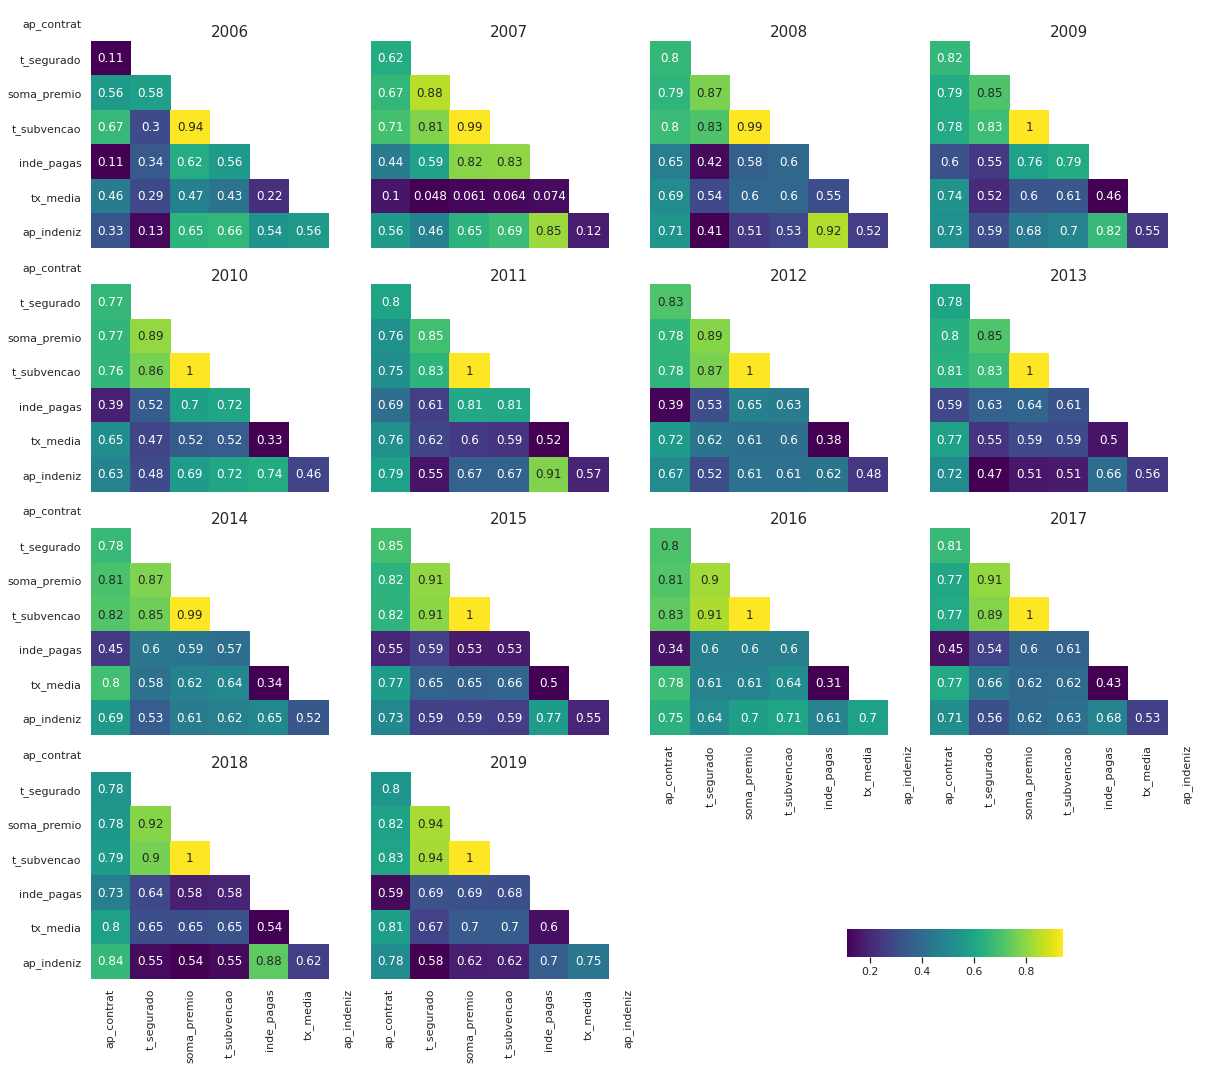
\includegraphics[width=0.9\textwidth]{figuras/corr_anos.png}
	\parbox{\dimexpr\linewidth-2cm}{\raggedright
    \strut \textsuperscript{Fonte: Elaboração própria}\strut}
    \label{corr_anos}
\end{figure}

Ao se analisar a Figura \ref{corr_anos}, é possível observar que há grupos de variáveis que apresentam uma maior correlação entre si. A variável que representa o total de subvenção concedida apresenta, em todos os anos, correlação alta com variáveis como o número de apólices contratadas, total segurado e a soma dos prêmios. Em particular, a correlação do total da subvenção com a soma dos prêmios é igual a $0,94$ no ano de $2006$ e, aproximadamente, igual a $1$ nos demais anos analisados. A correlação positiva entre o total de subvenção concedida e as variáveis relacionadas com o total segurado e o prêmio, indica que, assim como é apontado por Ferreira e Ferreira (2009), a participação do governo, por meio do subsídio concedido pelo PSR, é fundamental e deve garantir a sustentabilidade do seguro rural de forma a assegurar a estabilidade dos agricultores e demais participantes do sistema. 

Além disso, há uma alta correlação entre variáveis como o número de apólices contratadas e o total segurado, assim como entre o total segurado e o valor do prêmio. As variáveis que apresentaram menor correlação, embora ainda apresentem uma correlação positiva, são as variáveis que se relacionam com a ocorrência de sinistros, como o número de indenizações e total de das indenizações pagas. Estas variáveis apresentam, em todos os anos, menores correlações com as demais variáveis do conjunto de dados. 

\subsection{ANÁLISE DE COMPONENTES PRINCIPAIS} 

O gráfico da Figura \ref{var_ratio} apresenta a variância explicada acumulada pelos componentes principais para cada ano analisado. Neste gráfico é possível observar que o primeiro componente principal é responsável pela maior parte da variância explicada acumulada em todos os anos analisados. Ou seja, apenas o primeiro componente principal é capaz de fornecer informação sobre a variância de todo o conjunto de variáveis de seguro rural. 

\begin{figure}[H]
	\centering
	\caption{Variância explicada acumulada pelos componentes principais. Brasil $2006$ -- $2019$}
	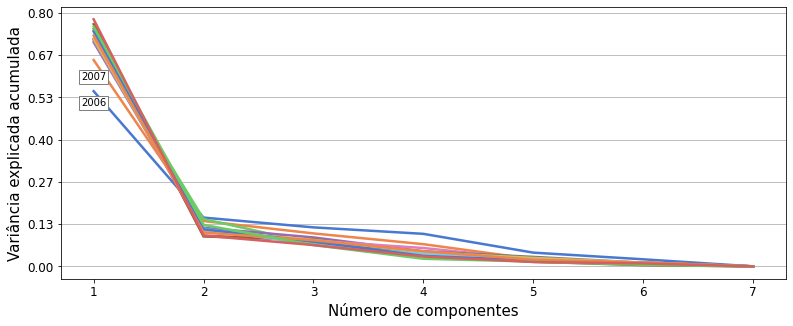
\includegraphics[width=0.8\textwidth]{figuras/var_radio.png}	\parbox{\dimexpr\linewidth-2cm}{\raggedright
    \strut \textsuperscript{Fonte: Elaboração própria}\strut}
    \label{var_ratio}
\end{figure}

É necessário ressaltar que, nos anos de $2006$ e $2007$ (destacados na Figura \ref{var_ratio}), a variância explicada acumulada pelo primeiro componente foi inferior a $0,72$, sendo igual à $0,55$ em $2006$ e $0,65$ em $2007$. No entanto, é possível considerar que a utilização dos escores do primeiro componente principal na análise exploratória de dados espaciais é adequada, pois o primeiro componente é capaz de representar, em média, $71,72\%$ da variabilidade dos dados originais \cite{everitt11}.

%\begin{figure}[H]
%	\centering
%	\caption{Diagrama de dispersão entre os dois primeiros componentes. Brasil $2006$ -- $2019$}
%	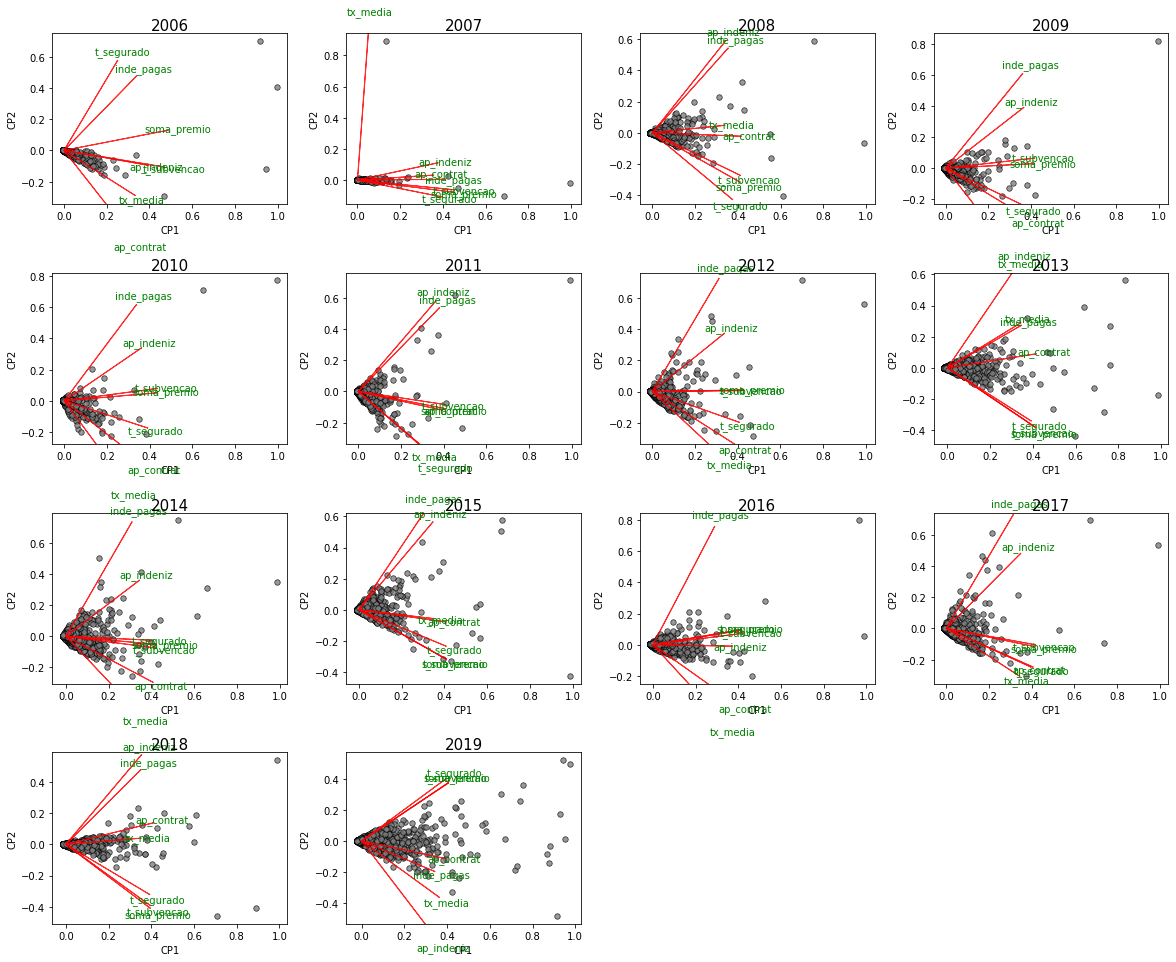
\includegraphics[width=1\textwidth]{figuras/acp_biplot.png}	\parbox{\dimexpr\linewidth-2cm}{\raggedright
%    \strut \textsuperscript{Fonte: Elaboração própria}\strut}
%    \label{acp_biplot}
%\end{figure}

A Figura \ref{corr_pca_var} ilustra o efeito das variáveis de seguro rural em cada um dos componentes principais. Quanto mais clara da cor do retângulo, mais próximo de $1$ é o valor do coeficiente, portanto, maior o grau de associação positiva entre os componentes principais e as variáveis. Por outro lado, quanto mais escura a cor do retângulo, menor é o valor do coeficiente, portanto, menor o grau de associação entre os componentes principais e as variáveis.


\begin{figure}[H]
	\centering
	\caption{Efeito das variáveis em cada componente. Brasil $2006$ -- $2019$.}
	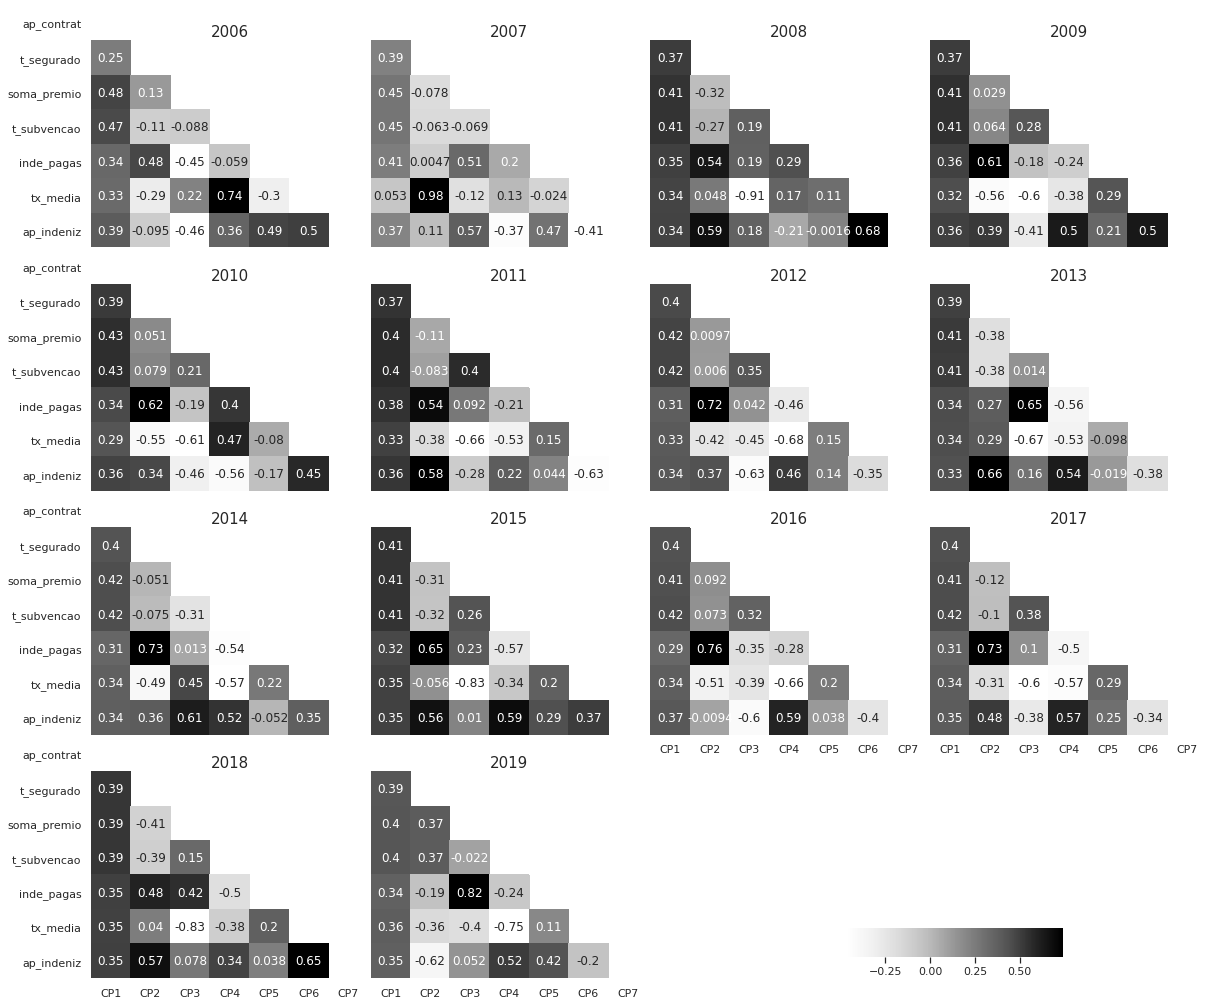
\includegraphics[width=0.9\textwidth]{figuras/corr_pca_var.png}	\parbox{\dimexpr\linewidth-2cm}{\raggedright
    \strut \textsuperscript{Fonte: Elaboração própria}\strut}
    \label{corr_pca_var}
\end{figure}

É possível constatar, através da Figura \ref{corr_pca_var}, que, em todos os anos entre $2006$ e $2019$, o primeiro componente principal é positivamente correlacionado com todas as variáveis do conjunto de dados. Além disso, a distribuição do efeito das variáveis no primeiro componente se dá de forma relativamente homogênea entre as variáveis analisadas, já que os valores dos coeficientes possuem valores semelhantes. 

Devido à estrutura de correlação entre as variáveis de seguro rural, foi possível utilizar os escores do primeiro componente principal como uma variável representativa das demais variáveis originais. Os escores do primeiro componente principal foram, em todos os anos, positivamente correlacionados com todas as variáveis originais. Além disso, em todos os anos analisados, a variância explicada acumulada pelo primeiro componente foi superior a 55,3\%. Sendo assim, o valor do escore do primeiro componente principal é representativo para resumir a informação sobre todas as variáveis de seguro rural aqui apresentadas. Quanto maior o valor desse escore para um município, maiores os valores das apólices, da importância segurada, dos prêmios etc.


\subsection{ANÁLISE EXPLORATÓRIA DE DADOS ESPACIAIS}

\subsubsection{Distribuição espacial dos escores do 1º componente principal}

O primeiro grupo de mapas, apresentado na Figura \ref{map_cp1}, exibe a distribuição espacial dos escores do primeiro componente principal nos municípios brasileiros entre os anos de $2006$ e $2019$. Por meio destes mapas, busca-se identificar visualmente se há a ocorrência de padrões na distribuição espacial no conjunto das variáveis do seguro rural representadas pelos escores do primeiro componente. Para a construção dos mapas, os valores da variável foram divididos em cinco intervalos através da utilização do algoritmo Fisher-Jenks aos valores das variáveis diferentes de $0$. Além disso, para tornar possível a comparação entre os anos, os intervalos foram criados tendo como referência os valores do ano de 2019 \cite{jenks77_2}

%\begin{figure}[H]
%	\centering
%	\caption{Distribuição espacial do primeiro componente principal. Brasil $2006$ -- $2019$.}
%	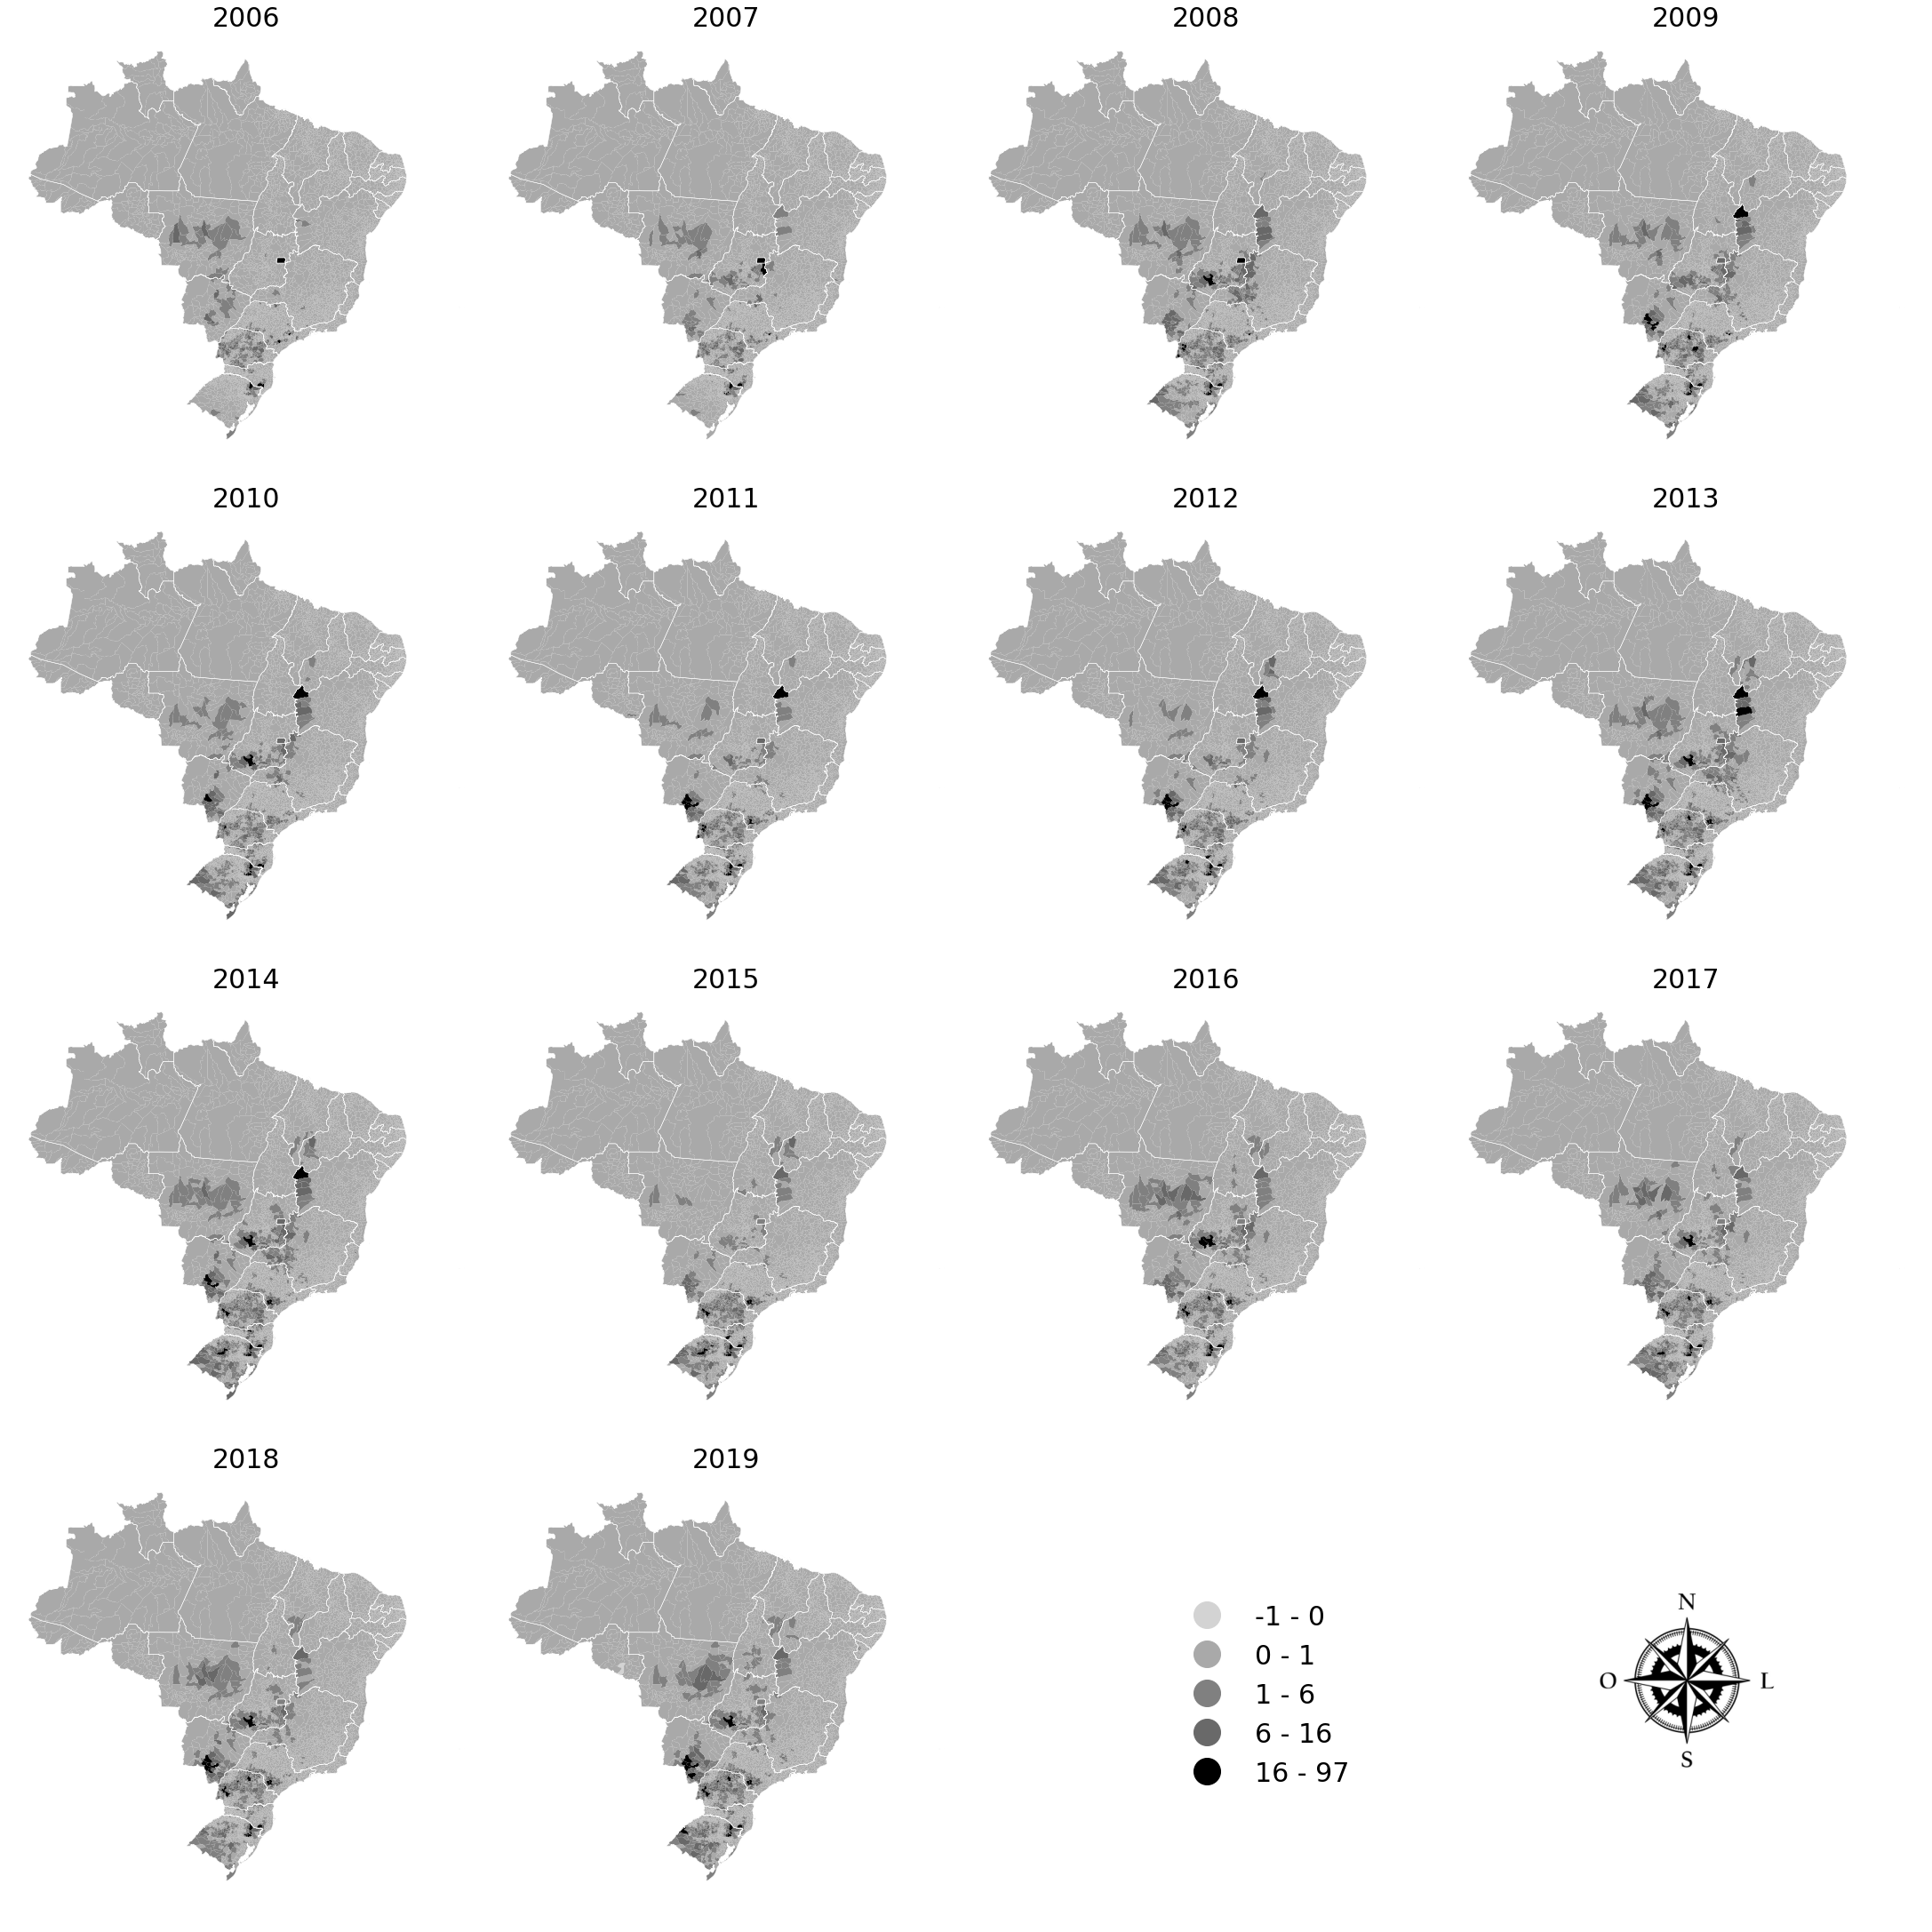
\includegraphics[width=0.9\textwidth]{figuras/map_CP1.png}	\parbox{\dimexpr\linewidth-2cm}{\raggedright
%    \strut \textsuperscript{Fonte: Elaboração própria}\strut}
%    \label{map_cp1}
%\end{figure}

\begin{figure}[H]
	\centering
	\caption{Distribuição espacial do primeiro componente principal. Brasil $2006$ -- $2019$.}
	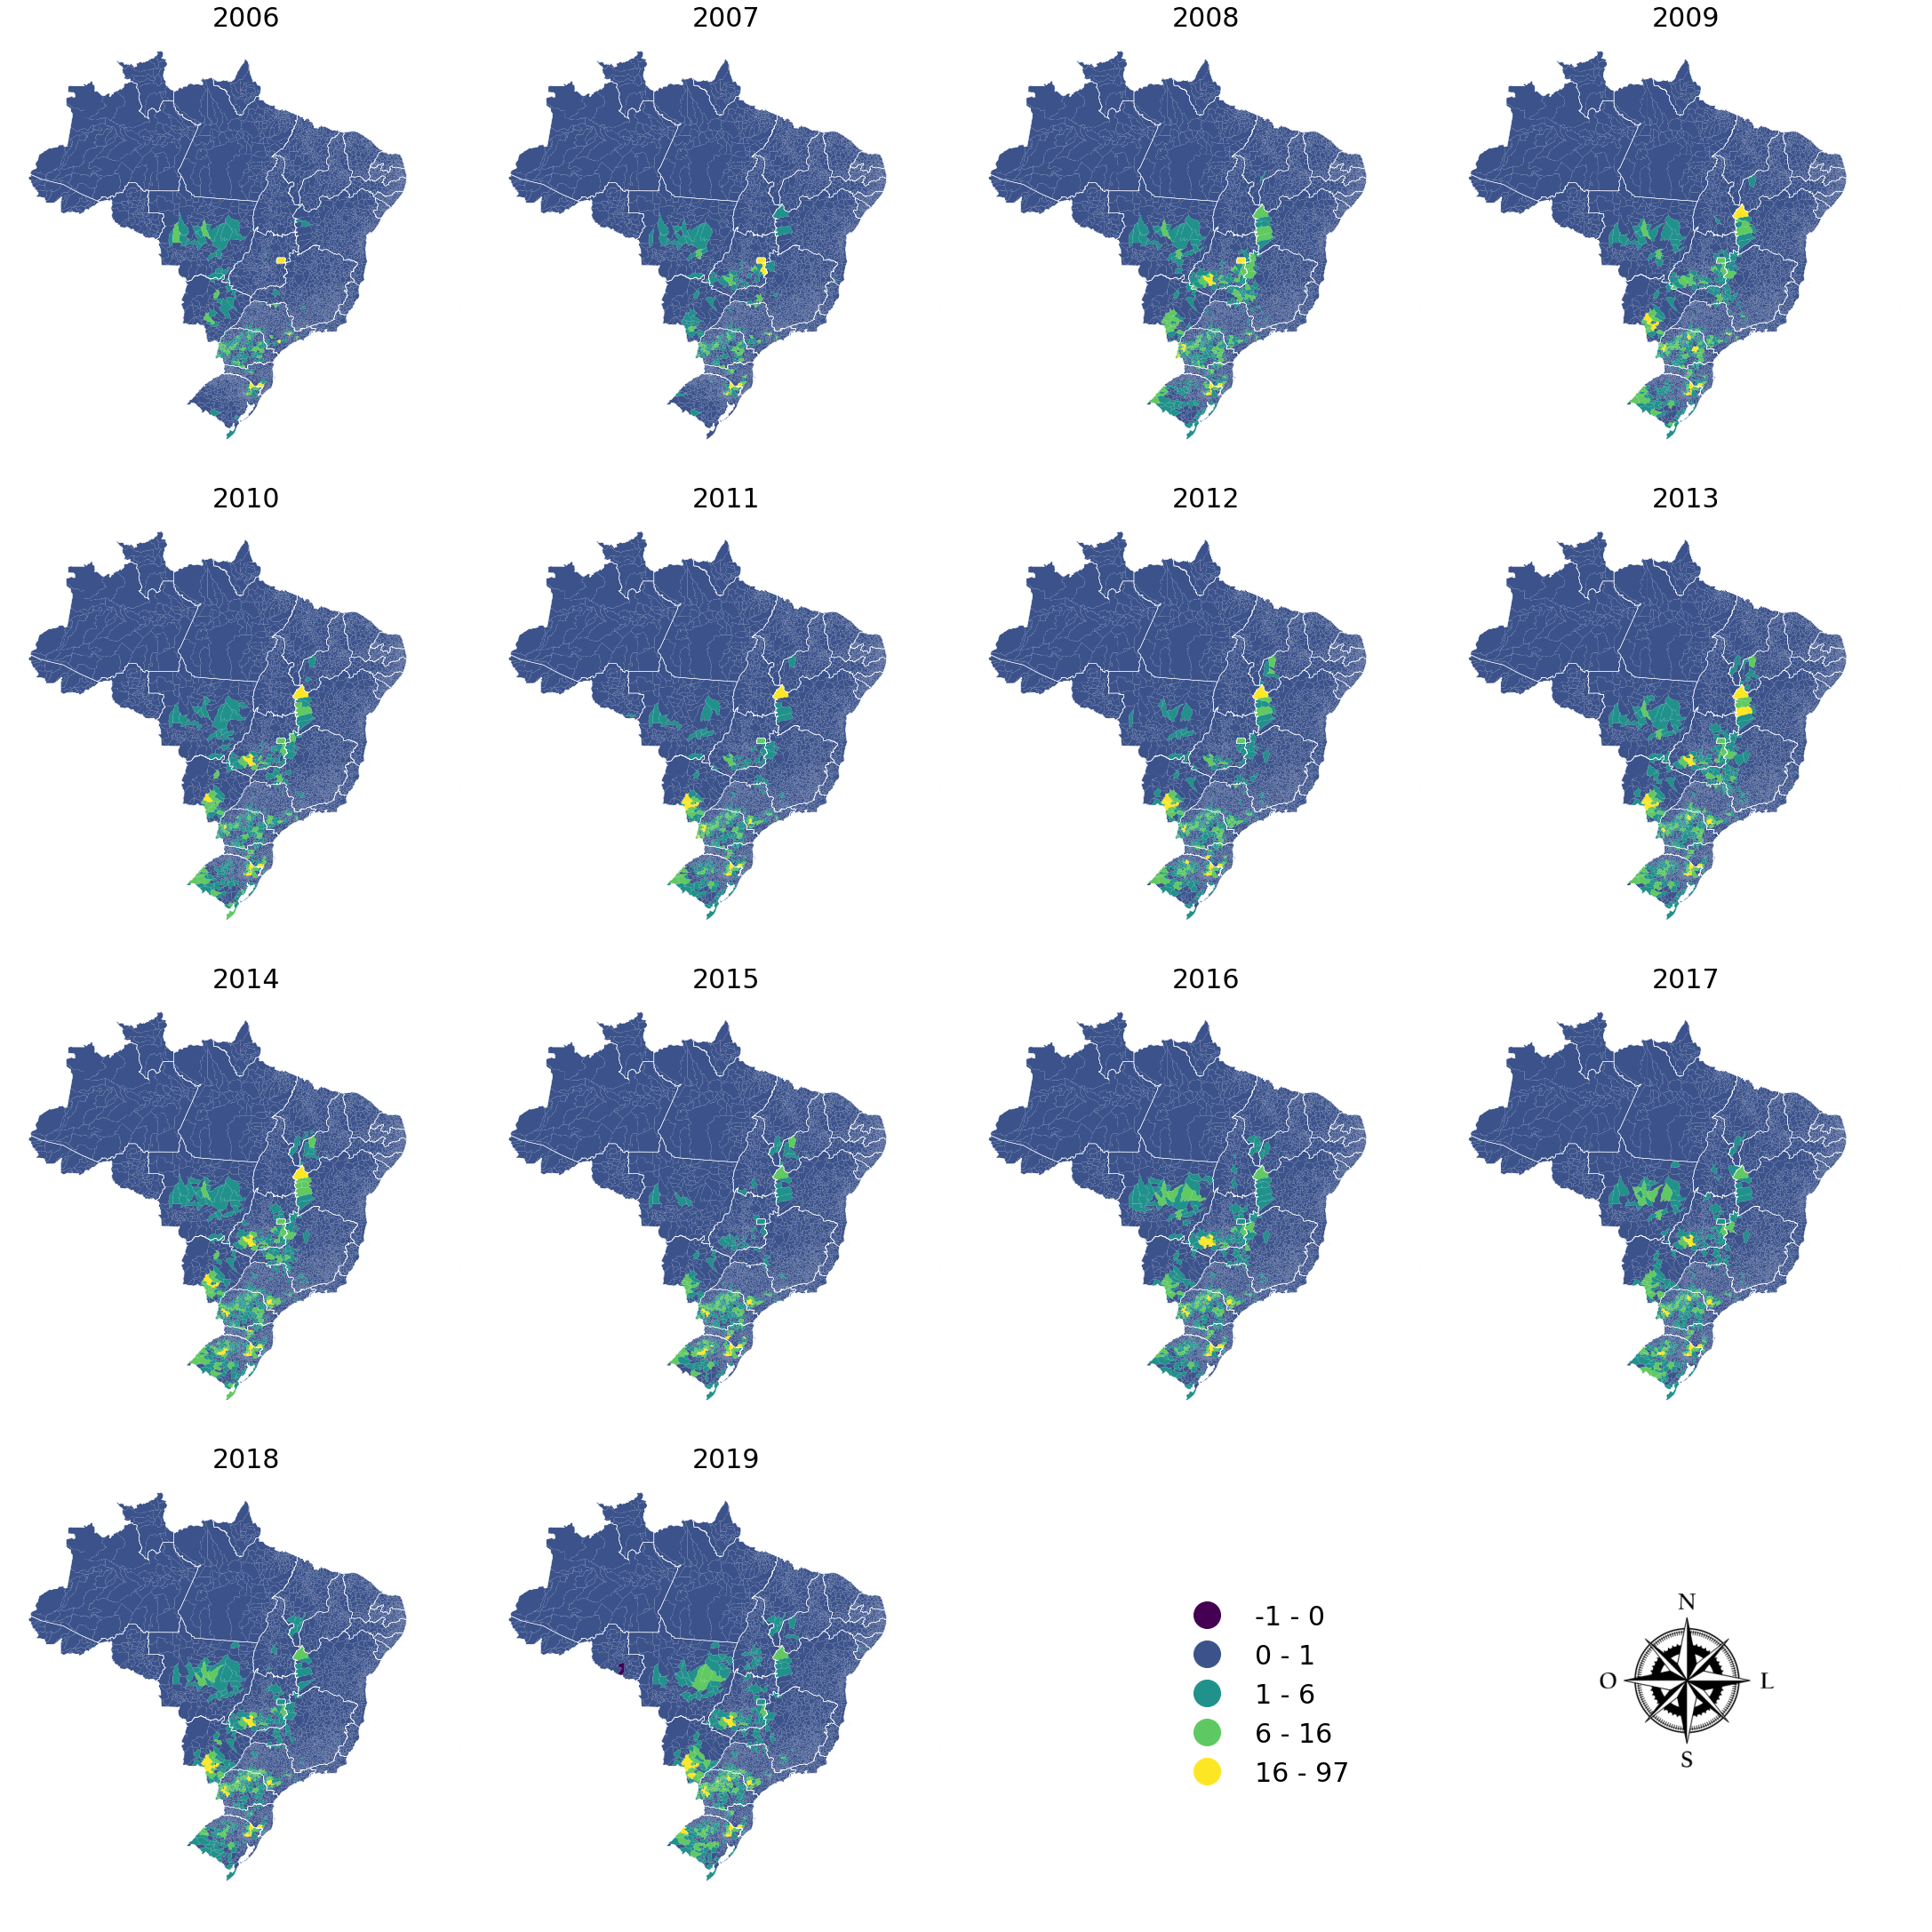
\includegraphics[width=0.9\textwidth]{figuras/map_CP1_color.png}	\parbox{\dimexpr\linewidth-2cm}{\raggedright
    \strut \textsuperscript{Fonte: Elaboração própria}\strut}
    \label{map_cp1}
\end{figure}

Pela análise da Figura \ref{map_cp1}, é possível observar que a distribuição espacial do seguro rural nos municípios brasileiros se modificou no decorrer dos anos, apesar de se concentrar principalmente nas Regiões Sul, Sudeste e Centro-Oeste. É possível também destacar que, durante o período analisado, há indícios de concentrações espaciais na região do Extremo Oeste Baiano no Estado da Bahia, Sudoeste de Mato Grosso do Sul, Sul Goiano no Estado de Goiás e Sudeste, no sul do Estado de São Paulo.

\subsubsection{Autocorrelação espacial global}

O valor do \textit{I} de Moran foi calculado utilizando-se dos escores do primeiro componente principal para todos os anos entre 2006 e 2019. Os resultados obtidos são apresentados na Figura \ref{i_moran_cp1}. %Todos os valores do \textit{I} de Moran foram estatisticamente significativos ao nível de significância de $5\%$. 

Ao se analisar o gráfico da Figura \ref{i_moran_cp1}, é possível observar que todos os valores do \textit{I} de Moran foram positivos e significativos (a média do \textit{I} de Moran foi de $0,46$ no período analisado). Este fato indica que há a presença de autocorrelação espacial positiva do seguro rural nos municípios brasileiros. Ou seja, o fato de um município possuir valores acima da média para as variáveis relacionadas ao seguro rural é influenciado, além de outros fatores, pelo valor desse conjunto de variáveis na região vizinha a este município. Dessa forma, o fato de um município possuir um valor da soma da importância segurada alta é influenciado, dentre outros fatores, pela soma da importância segurada nos municípios em seu entorno. O mesmo se aplica às variáveis soma dos prêmios, total da subvenção, soma das indenizações pagas, taxa média aplicada às apólices e número de apólices indenizadas. 

\begin{figure}[H]
	\centering
	\caption{Autocorrelação espacial (\textit{I} de Moran) do primeiro componente principal. Brasil $2006$ -- $2019$}
	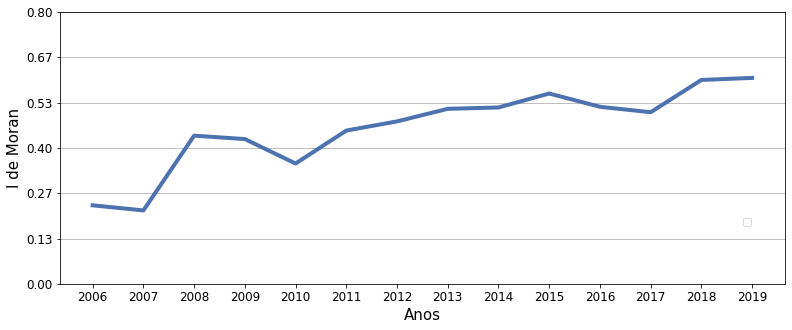
\includegraphics[width=0.8\textwidth]{figuras/i_de_moran_cp1.png}	\parbox{\dimexpr\linewidth-2cm}{\raggedright
    \strut \textsuperscript{Fonte: Elaboração própria.}\strut}\\
    \parbox{\dimexpr\linewidth-2.1cm}{\raggedright
    \strut \textsuperscript{Nota: Os valores do \textit{I} de Moran foram estatisticamente significativos em todas variáveis (valor$-p<0,005$)}\strut}
    \label{i_moran_cp1}
\end{figure}

Além da presença de autocorrelação positiva em todos os anos, a análise da Figura \ref{i_moran_cp1} indica que a dependência espacial apresentou um crescimento ao longo do período analisado. O menor valor de autocorrelação espacial observado é igual a $0,216$ em $2007$ e o maior valor ocorreu em $2019$ e foi igual a $0,606$. Entre os anos de $2006$ e $2019$, o valor da autocorrelação espacial apresentou um crescimento de cerca de $2,62$ vezes o valor observado em $2006$. Dessa forma, é possível inferir que, durante o período analisado, houve um aumento da autocorrelação espacial em todas as variáveis de seguro rural analisadas. 

\subsubsection{Autocorrelação espacial local}

Os mapas \textit{LISA} apresentados na Figura \ref{map_lisa_cp1} contêm $4$ grupos com diferentes características de associação espacial estatisticamente significativas para cada um dos anos analisados. No ano de $2006$, os agrupamentos do tipo AA, ou seja, agrupamentos formados por municípios cujas variáveis apresentavam valores altos e que possuíam vizinhos também com altos valores das variáveis de seguro rural, estavam concentrados exclusivamente nas regiões Centro-Oeste, Sudeste e Sul. A região Sul, em $2006$, possuía $74,56\%$ dos municípios do grupo AA, sendo que $64,32,\%$ destes pertenciam ao estado do Paraná, $6,43\%$  ao Rio Grande do Sul e $3,8\%$ à Santa Catarina.  

\begin{figure}[H]
	\centering
	\caption{Mapas \textit{LISA} para o primeiro componente principal.  Brasil $2006$ -- $2019$.}
	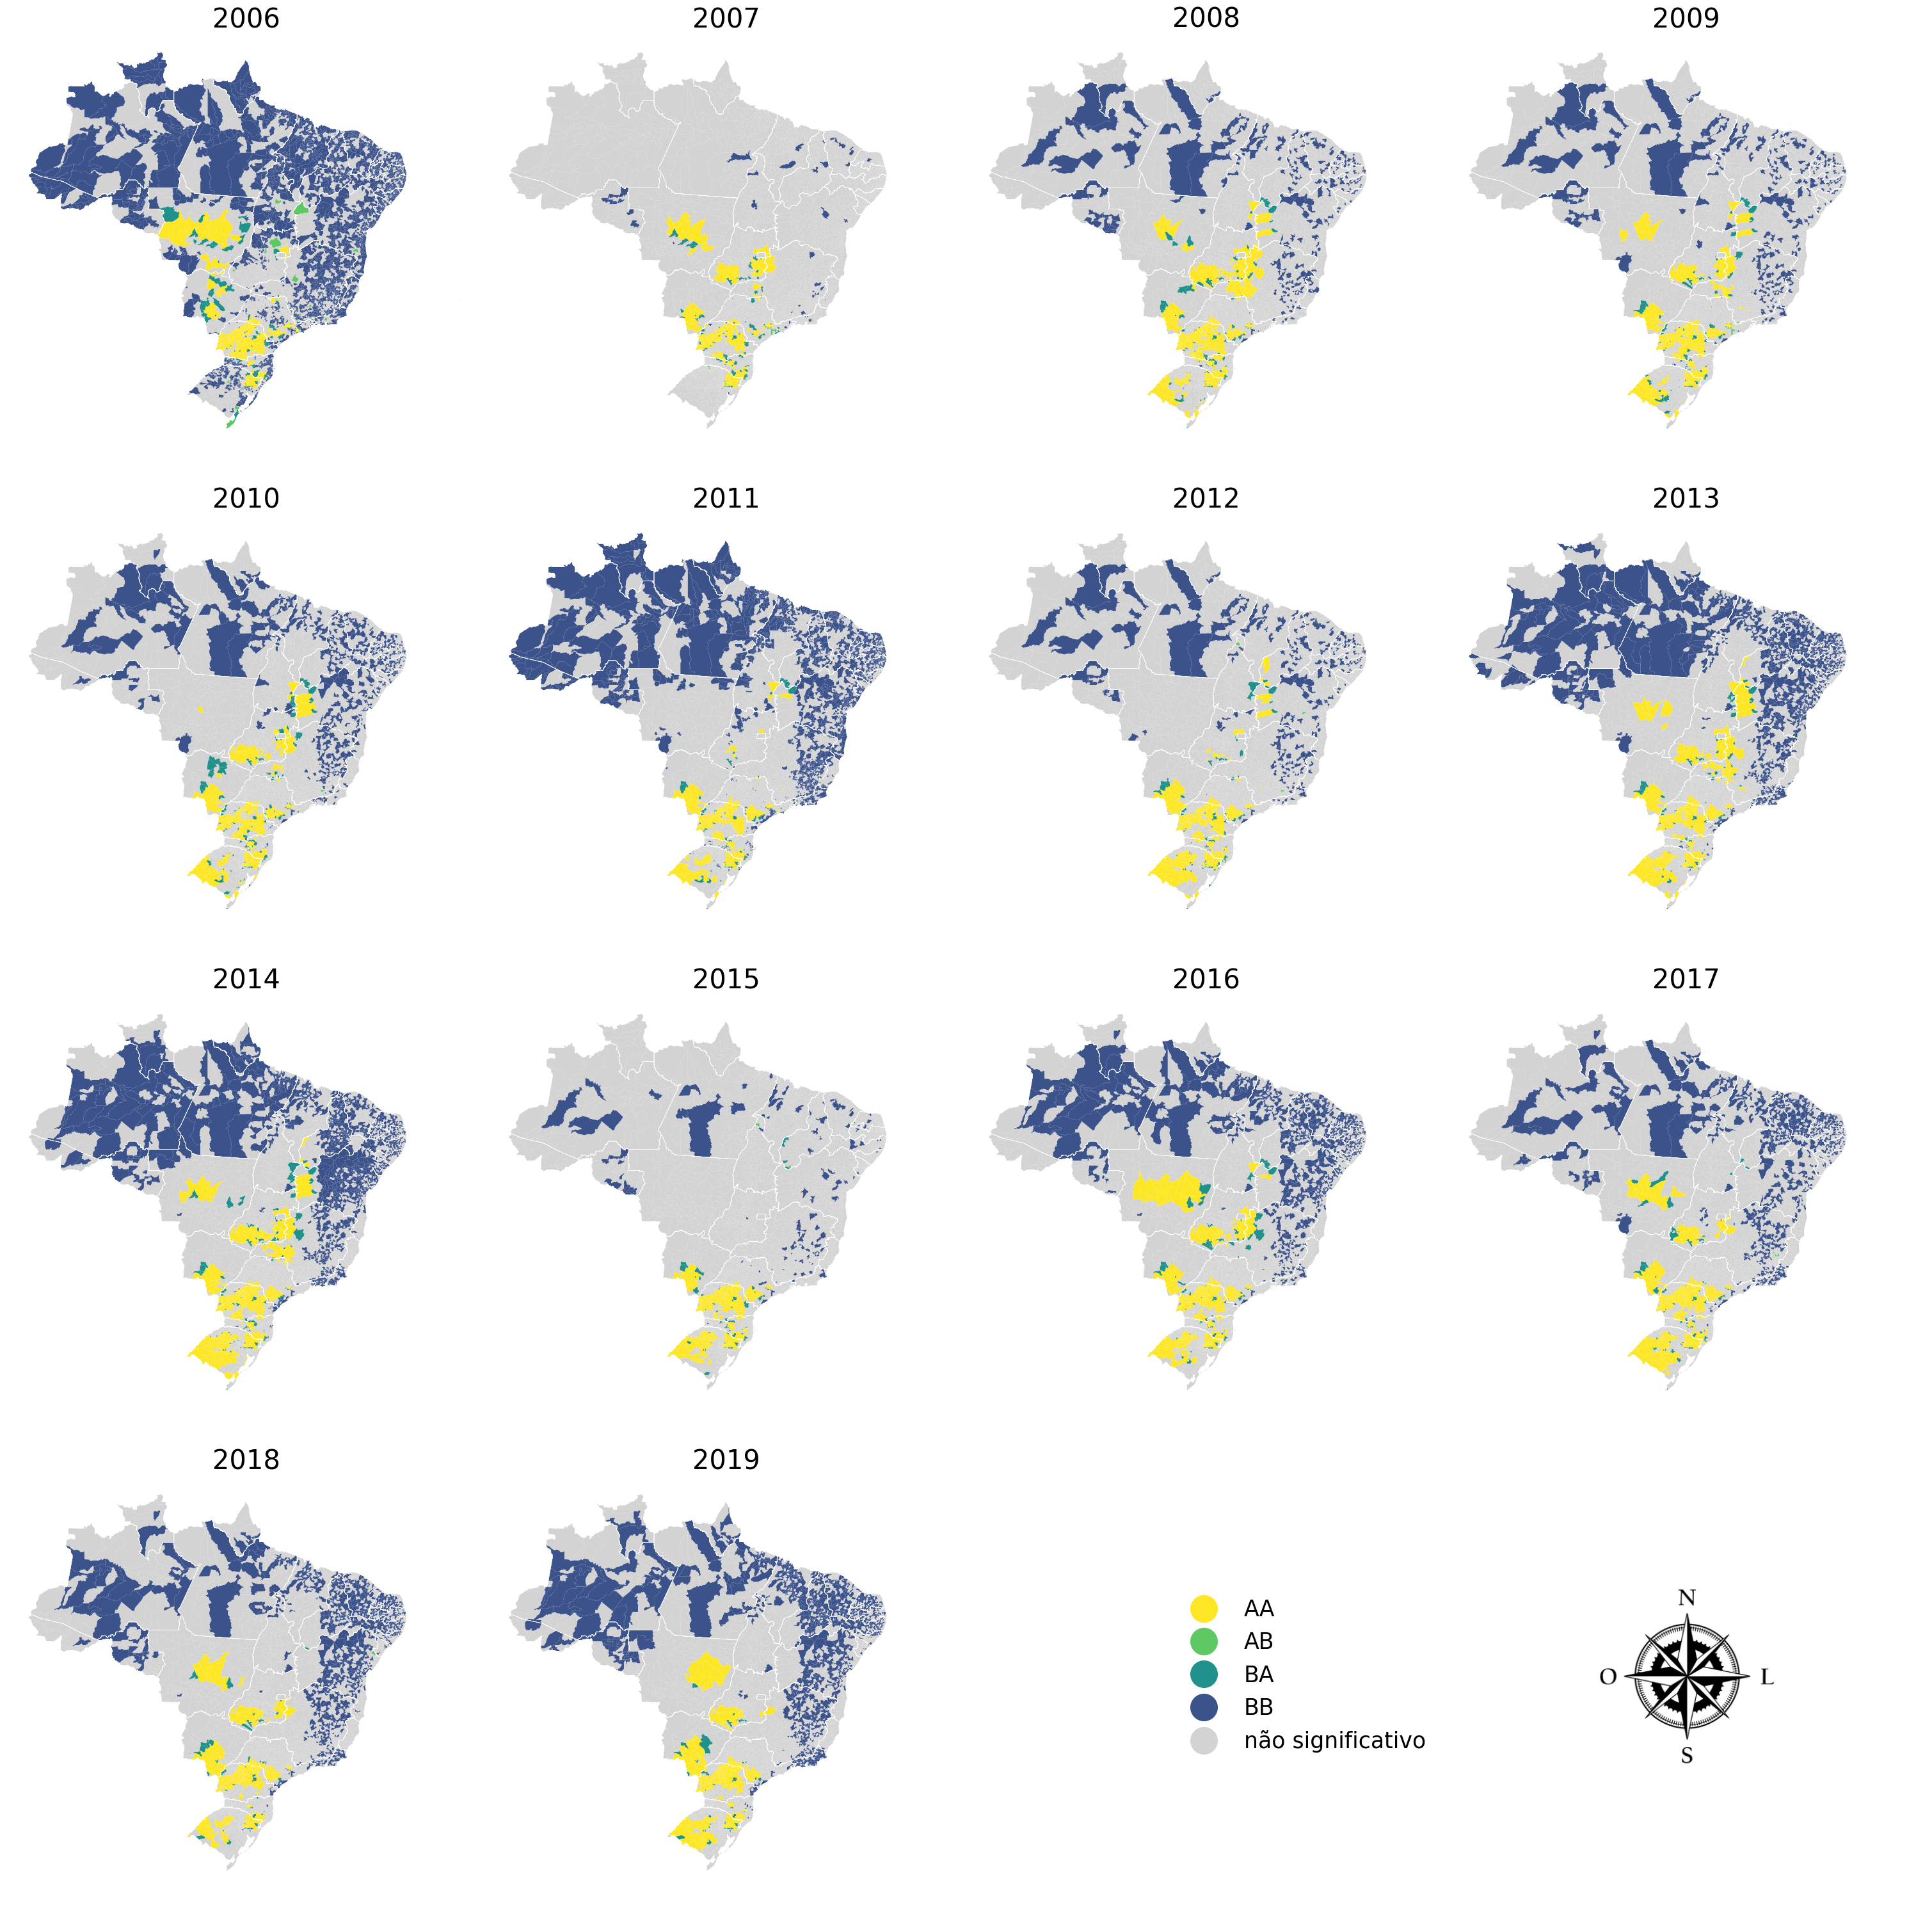
\includegraphics[width=0.9\textwidth]{figuras/map_lisa_cp1_viridis.png}\\
	\small \textsuperscript {Fonte: Elaboração própria.}
    \label{map_lisa_cp1}
\end{figure}

Na região Sudeste, em $2006$, cerca de $50$ municípios pertenciam ao estado de São Paulo, percentual correspondente à  $14,6\%$ dos municípios do agrupamento do tipo AA. Além disso, a região Centro-Oeste contava com cerca de $10,82\%$ dos municípios do grupo AA. O estado do Mato Grosso contava com $7,6\%$ dos municípios do grupo AA, o estado do Mato Grosso do Sul possuía $2,63\%$ dos municípios AA. 

Em $2019$, os municípios, cujo pertencimento ao grupo AA foi significativo, também se concentraram nas regiões Centro-Oeste, Sudeste e Sul. Mais especificamente, $8,10\%$ dos municípios do grupo AA estavam localizados no estado do Mato Grosso do Sul, $5,56\%$ se localizavam do estado de Goiás e $2,78\%$ no Mato Grosso. No Sudeste os municípios significativos do tipo AA se localizavam principalmente em São Paulo ($11,57\%$ do total), em Minas Gerais se localizavam apenas $0,46\%$ dos municípios AA.

A Região Sul, em $2019$, concentrava cerca de $79,86\%$ dos municípios do tipo AA significativos. A maior parte destes municípios ($48,61\%$) estava localizada no estado do Paraná, $19,67\%$ dos municípios do tipo AA pertenciam, em $2019$ ao estado do Rio Grande do Sul e, por fim, $3,24\%$ pertenciam ao estado de Santa Catarina. Além disso, vale destacar que os anos de $2007$ e $2015$, mesmo apresentando autocorrelação espacial positiva e significativa, apresentaram os menores números de municípios pertencentes ao grupo BB.

Segundo Santos e Silva (2017), historicamente, as apólices contratadas de seguro rural, o valor segurado e, por consequência, o valor de subvenção através do PSR se concentram regionalmente. Isto se dá devido à presença de maiores riscos de intempéries nos estados da Região Sul, em São Paulo e Minas Gerais. Estados como Mato Grosso do Sul, Mato Grosso, Goiás, e a região formada pelos estados do Maranhão, Tocantins, Piauí e Bahia, mais recentemente, também têm aderido aos contratos de seguro rural devido a fatores climáticos. 

Além disso, diversos fatores podem ser apontados como determinantes da concentração do mercado de seguro rural em poucas regiões, com poucas culturas, com participação reduzida de seguradoras. Segundo Santos, Sousa e Alvarenga (2013), alguns fatores que devem ser considerados são: o pequeno número e a discrepância no porte das seguradoras que ofertam esse tipo de seguro; dificuldades das instituições bancárias com operações no meio rural, levando a informações imprecisas e à elevação de riscos e preços; parcerias governamentais com operadores, como por exemplo, programas de crédito oficial operados pelo Banco do Brasil, que também é o controlador da maior seguradora agrícola;  o grau de oportunidade avaliado como pequeno pelas seguradoras, e por fim; o pequeno peso de parcerias e de avaliação das oportunidades envolvendo o segmento de corretagem.   

\section{CONSIDERAÇÕES FINAIS}

%O objetivo do presente trabalho foi analisar a distribuição espacial de dados multivariados do seguro rural nos municípios brasileiros entre os anos de $2006$ e $2019$. Além disso, buscou-se investigar a presença de padrões de distribuição espacial, por meio da autocorrelação espacial, bem como a existência de agrupamentos locais de distribuição espacial.

A partir da ACP, constata-se que a estrutura de correlação entre as variáveis de seguro rural possibilitou a utilização dos escores do primeiro componente principal como uma variável com a capacidade de representar o conjunto de variáveis de seguro rural disponível, em todos os anos analisados. A variância explicada acumulada pelo primeiro componente foi em média igual $71,72\%$. 

Os resultados da AEDE apontam que existe dependência espacial em todos os anos analisados, ou seja, existem padrões de associação espacial estatisticamente significativos nos dados de seguro rural. Também foi possível identificar a presença de \textit{clusters} espaciais significativos. Em geral, identificou-se que as maiores concentrações de apólices de seguro rural estão situadas nas regiões Sul, Centro-Oeste e Sudeste, no sul do Estado de São Paulo. 

Além disso, foi constatado que há um aumento na dependência espacial do seguro rural ao longo do período analisado. Ou seja, municípios que possuem uma maior adesão ao seguro rural tendem a ser geograficamente próximos de municípios que também têm maior adesão ao seguro rural. No entanto, a análise dos mapas \textit{LISA} indica que a concentração espacial  do tipo AA do seguro rural pouco se modificou no decorrer dos anos. 

%por meio da autocorrelação espacial, bem como a existência de agrupamentos locais de distribuição espacial.
%Os resultados da AEDE apontam que existe dependência espacial em todos os anos analisados. Ou seja, existem padrões de associação espacial estatisticamente significativos. Também foi possível identificar a presença de \textit{clusters} espaciais significativos. Tal resultado é observado em todas as variáveis de seguro rural analisadas. 
% Além disso, foi constatado que há um aumento na dependência espacial do seguro rural ao longo do período analisado. Ou seja, municípios que possuem uma maior adesão ao seguro rural tendem a ser geograficamente próximos de municípios que também têm maior número de apólices de seguro rural contratadas.

\newpage
\addcontentsline{toc}{section}{\hspace*{\distnumber}REFERÊNCIAS}
\begin{center}
\section*{REFERÊNCIAS} 
\end{center}
